\documentclass[Protokollheft.tex]{subfiles}
\begin{document}
\chapter{HF-Zeitbereich 1: Leapfrog}
%--------------- Start Vorbereitungsaufgaben ---------------
\section{Vorbereitungsaufgaben}



% --> Aufgabe
\begin{framed}
	\noindent \textbf{1.} Geben Sie~(6.6) und~(6.7) für $\Mkap \neq 0$ an. Ersetzen Sie die Ableitungen aus~(6.4) und~(6.5) mit dem zentralen Differenzenquotienten.\label{exer:updateSchemeNoConductor}
\end{framed}

Mit dem zentralen Differenzenquotient
\begin{equation*}
	\frac{\text{d}y}{\text{d}t}=\frac{y^{(n+1)}-y^{(n-1)}}{2\Delta t}
\end{equation*}
ergibt sich (6.6) zu
\begin{eqnarray*}
	\frac{\hfit^{(n+1)}-\hfit^{(n-1)}}{2\Delta t}&=&-\Mmui\curlfit\efit^{(n)}\\
	\hfit^{(n+1)}&=&\hfit^{(n-1)}-2\Delta t\Mmui\curlfit\efit^{(n)}.
\end{eqnarray*}
(6.7) ergibt sich mit dem zentralen Differenzenquotienten zu
\begin{eqnarray*}
	\frac{\efit^{(n+1)}-\efit^{(n-1)}}{2\Delta t}&=&-\Meps^{-1}\Mkap\efit^{(n)}+\Meps^{-1}(\curldfit\hfit^{(n)}-\jfit^{(n)})\\
	\efit^{(n+1)}&=&\efit^{(n-1)}-2\Delta t(\Meps^{-1}\Mkap\efit^{(n)}+\Meps^{-1}(\curldfit\hfit^{(n)}-\jfit^{(n)}))
\end{eqnarray*}

% --> Aufgabe
\begin{framed}
	\noindent \textbf{2.} Leiten Sie die Update-Gleichungen~(6.10) und~(6.11) des Leapfrog-Algorithmus ebenfalls für ${\Mkap \neq 0}$ her und erklären Sie, welche Schwierigkeiten hier auftreten.\label{exer:updateSchemeWithConductor}
\end{framed}

Um Update-Gleichungen erzeugen zu können nimmt man
\begin{eqnarray}
	\frac{\text{d}\hfit}{\text{d}t}\big |^{(m+\frac{1}{2})}&\approx&	\frac{\hfit^{(m+1)}-\hfit^{(m)}}{\Delta t}\\
	\frac{\text{d}\efit}{\text{d}t}\big |^{(m+1)}&\approx&	\frac{\efit^{(m+\frac{3}{2})}-\efit^{(m+\frac{1}{2})}}{\Delta t}	
\end{eqnarray}
an. Setzt man diese Annahme in die Gleichungen für $\hfit^{(n+1)}$ und $\efit^{(n+1)}$ ein so erhält man die Updategleichungen
\begin{eqnarray*}
	\hfit^{(m+1)}&=&\hfit^{(m-1)}-2\Delta t\Mmui\curlfit\efit^{(m+\frac{1}{2})}\\
	\efit^{(m+\frac{3}{2})}&=&\efit^{(m+\frac{1}{2})}-2\Delta t(\Meps^{-1}\Mkap\efit^{(m+1)}+\Meps^{-1}(\curldfit\hfit^{(m+1)}-\jfit^{(m+1)})).
\end{eqnarray*}

% --> Aufgabe
\begin{framed}
	\noindent \textbf{3.} Fertigen Sie eine Skizze mit zwei gleichen, zur Illustration aber zeichnerisch getrennten Zeitachsen an. Auf eine der Zeitachsen soll die elektrische Gitterspannung \efit, auf die andere Zeitachse die magnetische Gitterspannung \hfit\ zu den nach dem Leapfrog-Verfahren jeweils definierten Zeitpunkten aufgetragen werden. Veranschaulichen Sie anschließend das Leapfrog-Verfahren mithilfe von Pfeile, indem Sie eintragen, welche Größen an welchen Zeitschritten in die jeweils zeitlich folgenden Größen eingehen.\label{exer:LeapfrogOnTimeAxes}
\end{framed}
\noindent
Die grafische Darstellung des Leapfrog-Algorithmus ist in Abbildung \ref{fig:zeitachse} zu sehen.
\begin{figure}[h]
	\centering
	\def\svgwidth{0.7\textwidth}
	\input{zeitachse.pdf_tex}
	\caption{Grafische Darstellung des Leapfrog-Verfahrens}
	\label{fig:zeitachse}
\end{figure}

% --> Aufgabe
\begin{framed}
	\noindent \textbf{4.} Für eine homogene Materialverteilung und äquidistante Gitter
    lässt sich eine Abschätzung des größten Eigenwertes von $\Amat'$ (gegeben durch~(6.27)) mit der Spaltensummennorm angeben, sodass~
    \begin{align}
        \lambda_{\text{max}} \approx\|\Amat'\|_1=\max_{k=1,\ldots,n} \sum_{i=1}^n |a_{ik}|,
    \end{align}
    wobei $\Amat'$ eine quadratische Matrix mit $n$ Spalten und $n$ Zeilen
    ist. Schätzen Sie mithilfe dieser Spaltensummennorm\footnote{Im Allgemeinen würde man hier die Abschätzung von $\lambda_{\text{max}}\approx\|\Amat'\|_2\le\sqrt{\|\Amat\|_1\|\Amat\|_\infty}$ mithilfe der Spektralnorm durchführen. Für symmetrische Matrizen $\Amat$ wäre diese Abschätzung sogar exakt. Da die Berechnung der Spektralnorm sehr aufwändig sein kann, wird diese üblicherweise wie angegeben abgeschätzt. Da $\Amat'$ schiefsymmetrisch ist, gilt hier außerdem ${\|\Amat\|_2\le\|\Amat\|_1=\|\Amat\|_\infty}$ und die Abschätzung kann genauso gut mit der Spalten- bzw. Zeilensummennorm vorgenommen werden.}
    den größten Eigenwert von $\Amat'$ für ein äquidistantes Gitter mit
    homogener Materialfüllung und unter Vernachlässigung von Randeffekten ab. Geben Sie für diesen Fall $\Delta t_{\text{max}}$ an.\label{exer:approxEVofAprime}
\end{framed}

\emph{Fügen Sie hier Ihre Lösung ein}

% --> Aufgabe
\begin{framed}
	\noindent \textbf{5.} Gehen Sie wie in der vorherigen Aufgabe vor, jedoch benutzen Sie
    dieses Mal die Matrix $\Amat$ um $\Delta t_{\text{max}}$ abzuschätzen. Verwenden Sie hierfür~(6.18).\label{exer:approxEVofA}
\end{framed}

\emph{Fügen Sie hier Ihre Lösung ein}

% --> Aufgabe
\begin{framed}
	\noindent \textbf{6.} Für Rechengebiete mit $n_z=2$ und elektrischen
    Randbedingungen sind die $x$- und $y$-Komponenten von $\Meps$ sowie die
    $z$-Komponente von $\Mmui$ gleich Null. Schätzen Sie für diesen Fall,
    unter sonst gleichen Bedingungen wie zuvor, $\Delta t_{\text{max}}$ aus
    der Spaltensummennorm von $\Amat'$ ab.\label{exer:approxDeltaTmax}
\end{framed}

\emph{Fügen Sie hier Ihre Lösung ein}

% --> Aufgabe
\begin{framed}
	\noindent \textbf{7.} Berechnen Sie mithilfe des CFL Kriteriums~(6.32) die maximale
    Zeitschrittweite $\Delta t_{\text{max}}^{\text{CFL}}$ für $\Delta x=\Delta
    y=\Delta z=1, \eps_\text{r}=1$ und $\mu_\text{r}=1$.\label{exer:deltaTmaxCFL}
\end{framed}

\emph{Fügen Sie hier Ihre Lösung ein}

\section{Aufgaben während der Praktikumssitzung}
In diesem Versuch soll die Stabilität des Leapfrog-Algorithmus' anhand eines einfachen Beispiels untersucht werden.
Als Beispiel dient die Ausbreitung einer im Freiraum ($\eps_\text{r}=1$, $\mu_\text{r}=1$) linienförmig angeregten 2D-Welle (Zylinderwelle). Als Rechengebiet soll dafür ein Würfel mit Kantenlänge 1 gewählt werden. Es sollen drei verschiedene Gitter, gegeben durch
\begin{itemize}
    \item $n_x=11$, $n_y=11$, $n_z=2$,
    \item $n_x=41$, $n_y=41$, $n_z=2$,
    \item $n_x=91$, $n_y=91$, $n_z=2$,
\end{itemize}
für die Stabilitätsuntersuchung verwendet werden. Um eine Welle zu erzeugen, muss die Welle im Rechengebiet angeregt werden. Dies soll mit Hilfe eines
Linienstromes in der Mitte des Rechengebietes erfolgen, wie in
Abbildung~\ref{fig:anregung} dargestellt.\\

\begin{figure}[h]
    \centering
    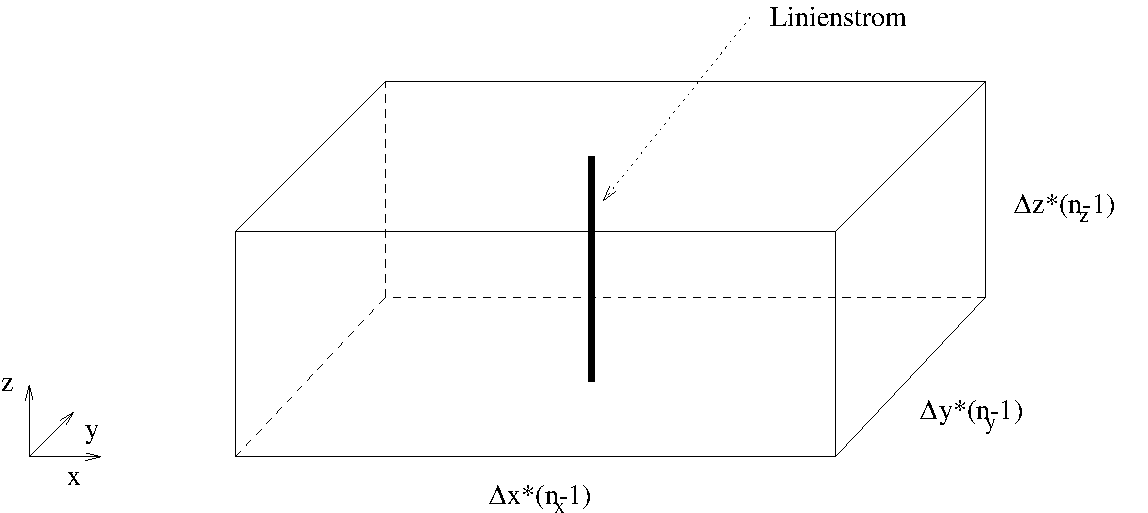
\includegraphics[scale=0.7]{v6_praktskizze.pdf}
    \caption{Geometrie des Rechengebietes}\label{fig:anregung}
\end{figure}

\noindent Dieser Linienstrom soll den zeitlichen Verlauf
\begin{align}
    \jfit(t) = \jfit_{\text{max}} \exp{-4\left(\frac{t-\sigma_t}{\sigma_t}\right)^2}
\end{align}
besitzen. Mit $\sigma_t=\SI{6e-10}{s}$ und $0 < t\leq 2 \sigma_t$ wird das Gebiet also für eine bestimmte Zeit gaußförmig angeregt. Wenn Sie noch Zeit haben, können Sie z.B. auch eine harmonische oder konstante Anregung implementieren, dies sei Ihnen jedoch freigestellt.\\
\noindent
Wie im Theorieteil erläutert wurde, existiert bei expliziten Zeitschrittverfahren eine maximale Zeitschrittweite, bis zu
der das System noch stabil ist. Wird diese Zeitschrittweite
überschritten, so divergieren die Werte für {\efit} und {\hfit}. Die maximale
Zeitschrittweite soll durch drei verschiedene Methoden gefunden werden. Nutzen Sie bitte für die Implementierungen das teilweise vorgegebene Skript \lstinline{versuch6.m}.

% --> Aufgabe
\begin{framed}
	\noindent \textbf{1.} \textbf{CFL-Kritierium}\\
Bestimmen Sie für alle drei Gitter den maximal möglichen Zeitschritt anhand des CFL-Kriterium.\label{exer:calcDeltaTmaxWithCFL}
\end{framed}

%\emph{Fügen Sie hier Ihre Lösung ein}
Mithilfe des CFL-Kriteriums bestimmen sich die Maximalen Zeitschritte zu $2.352755\cdot 10^{-10}$ s für $n_x = n_y = 11$, $5.895652 \cdot 10^{-11}$ s für $n_x = n_y = 41$ und $2.620618 \cdot 10^{-11}$ s für $n_x = n_y = 91$
% --> Aufgabe
\begin{framed}
	\noindent \textbf{2.} \textbf{Stabilitätsuntersuchung mithilfe der Systemmatrix}\\
Die maximale Zeitschrittweite soll nach Gleichung~(6.31) bestimmt werden.
Der größte Eigenwert einer Systemmatrix A kann mit Hilfe
des Matlab-Befehls\\
\lstinline{[Eigenvektoren,Eigenwerte] = eigs(A,1)} gefunden werden.\label{exer:calcDeltaTmaxWithEV}
\end{framed}

%\emph{Fügen Sie hier Ihre Lösung ein}
Mit der Eigenwertbestimmung der Systemmatrizen kommt für den Fall $n_x=n_y =11$ eine maximale Zeitschrittweite von $2.388030 \cdot 10^{-10}$ s. Für $n_x=n_y=41$ führt dies auf eine Zeitschrittweite von $5.901125\cdot 10^{-11} $ s. Im Falle von $n_x=n_y=91$ kommt der Rechner zu keinem Ergebnis. 

% --> Aufgabe
\begin{framed}
	\noindent \textbf{3.} \textbf{Experimentelle Bestimmung mithilfe der Energie des Systems}\\
Implementieren Sie hierzu zuerst ein Programm, das mit Hilfe des Leapfrog-Algorithmus den
zeitlichen Verlauf eines elektromagnetischen Feldproblems ausgibt,
also aus den jeweils alten Werten von $\efit$ und $\hfit$ die neuen
berechnet. Hierfür muss zusätzlich die Funktion
\begin{align}
    \left[\hfit^{(m+1)},\efit^{(m+\frac{3}{2})}\right]= {\text{leapfrog}}
	\left(\hfit^{(m)},\efit^{(m+\frac{1}{2})},\jfit^{(m+1)},\Mmui,\Meps^{-1},\curlfit,\curldfit,\Delta t \right)
\end{align}
für das Leapfrog-Update in jedem Zeitschritt implementiert werden.
Finden Sie anschließend durch Ausgeben der Gesamtenergie (Gleichung~(6.34))
in jedem Zeitschritt den maximal möglichen Zeitschritt des Verfahrens.
Überlegen Sie sich dazu, wie sich die Energie verhält, wenn das Verfahren instabil ist.
Vernachlässigen Sie dazu bei der Bestimmung der Energie zunächst, dass $\efit$
und $\hfit$ nicht zum gleichen Zeitpunkt definiert sind\footnote{Da
hier der exakte Werte für die Energie nicht interessant ist,
sondern nur untersucht werden soll, ob die Energie divergiert, ist
diese Näherung zulässig.}.\label{exer:calcDeltaTmaxWithEnergy}
\end{framed}

\emph{Fügen Sie hier Ihre Lösung ein}

\noindent Nun sollen die gefundenen maximalen Zeitschrittweiten für die verschiedenen Gitter verglichen und interpretiert werden.

% --> Aufgabe
\begin{framed}
	\noindent \textbf{4.} Erstellen Sie für den Vergleich eine Tabelle und kommentieren Sie, welche die exakteste Methode ist. Von welchen Parametern hängt die maximale Zeitschrittweite ab? Hat die Anregung einen Einfluss auf die Stabilität des Zeitschrittverfahrens?\label{exer:compareMethods4deltaTmax}
\end{framed}

\emph{Fügen Sie hier Ihre Lösung ein}

% --> Aufgabe
\begin{framed}
	\noindent \textbf{5.} Anstelle der Energie soll auch der Betrag des E-Feldes grafisch nach jedem Zeitschritt ausgegeben werden.
Somit erhält man den zeitlichen Verlauf einer sich in $x$- und $y$-Richtung
ausbreitenden Welle. Wählen Sie die Simulationszeit so, dass die Welle den Rand des Rechengebietes gerade noch nicht erreicht und speichern Sie sich den Plot des Feldes nach dem letzten Zeitschritt für die Ausarbeitung. Interpretieren Sie die Ergebnisse.\label{exer:visualizeWave}
\end{framed}

\emph{Fügen Sie hier Ihre Lösung ein}

% --> Aufgabe
\begin{framed}
	\noindent \textbf{6.} Bestimmen Sie nun die Energie mithilfe einer geeigneten Mittelung (siehe Abschnitt 6.2.4) und erstellen Sie einen Plot, der die Energieerhaltung verdeutlicht. Warum sinkt die Energie nach Erreichen des Maximalwertes wieder ab?\label{exer:energyConservation}
\end{framed}

In Abb. \ref{fig:enegiedesfeldes} ist deutlich der zeitlich etwas versetzte Anstieg der Energie mit zunehmender Anregung zu erkennen. Da sich eine Welle vom Leiter löst, folgt die Energie dem abnehmenden Anregestrom nur teilweise und strebt einem konstanten Wert zu. 

\begin{figure}
	\centering
	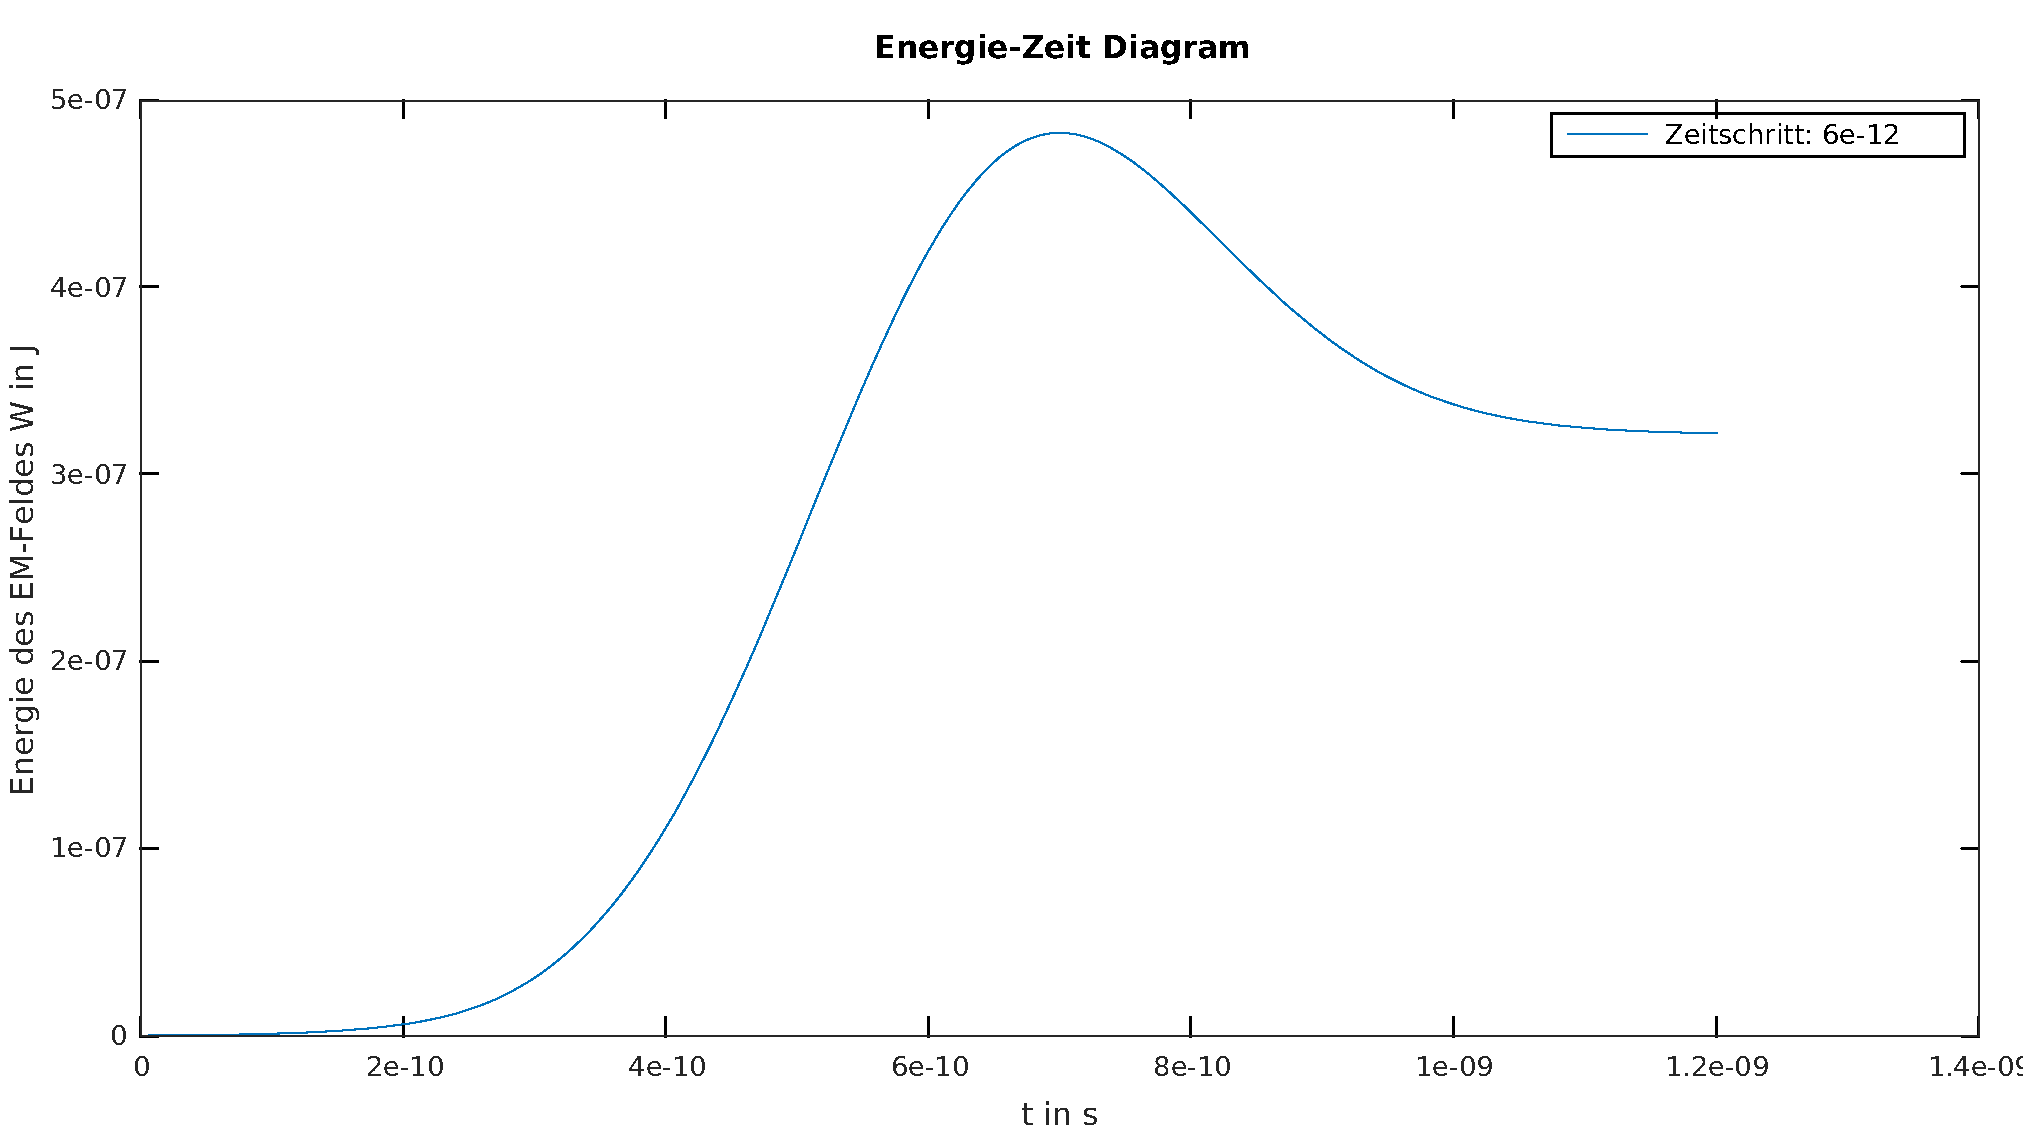
\includegraphics[width=0.7\linewidth]{EnegiedesFeldes}
	\caption{Energie der Zylinderwelle}
	\label{fig:enegiedesfeldes}
\end{figure}



%\emph{Fügen Sie hier Ihre Lösung ein}

% --> Aufgabe
\begin{framed}
	\noindent \textbf{7.} Bestimmen Sie abschließend die Leistung der Quelle und des Gesamtsystems und stellen Sie beide Größen in einem Plot dar.\label{exer:powerPlot}
\end{framed}


 Wie in Abb. \ref{fig:leistung} deutlich zu erkennen verhält sich die Leistung der Zylinderwelle entgegengesetzt zu der der Anregung. In dieser Folge ist die Leitung des Gesamtsystems nach außen ausgeglichen. 
\begin{figure}
	\centering
	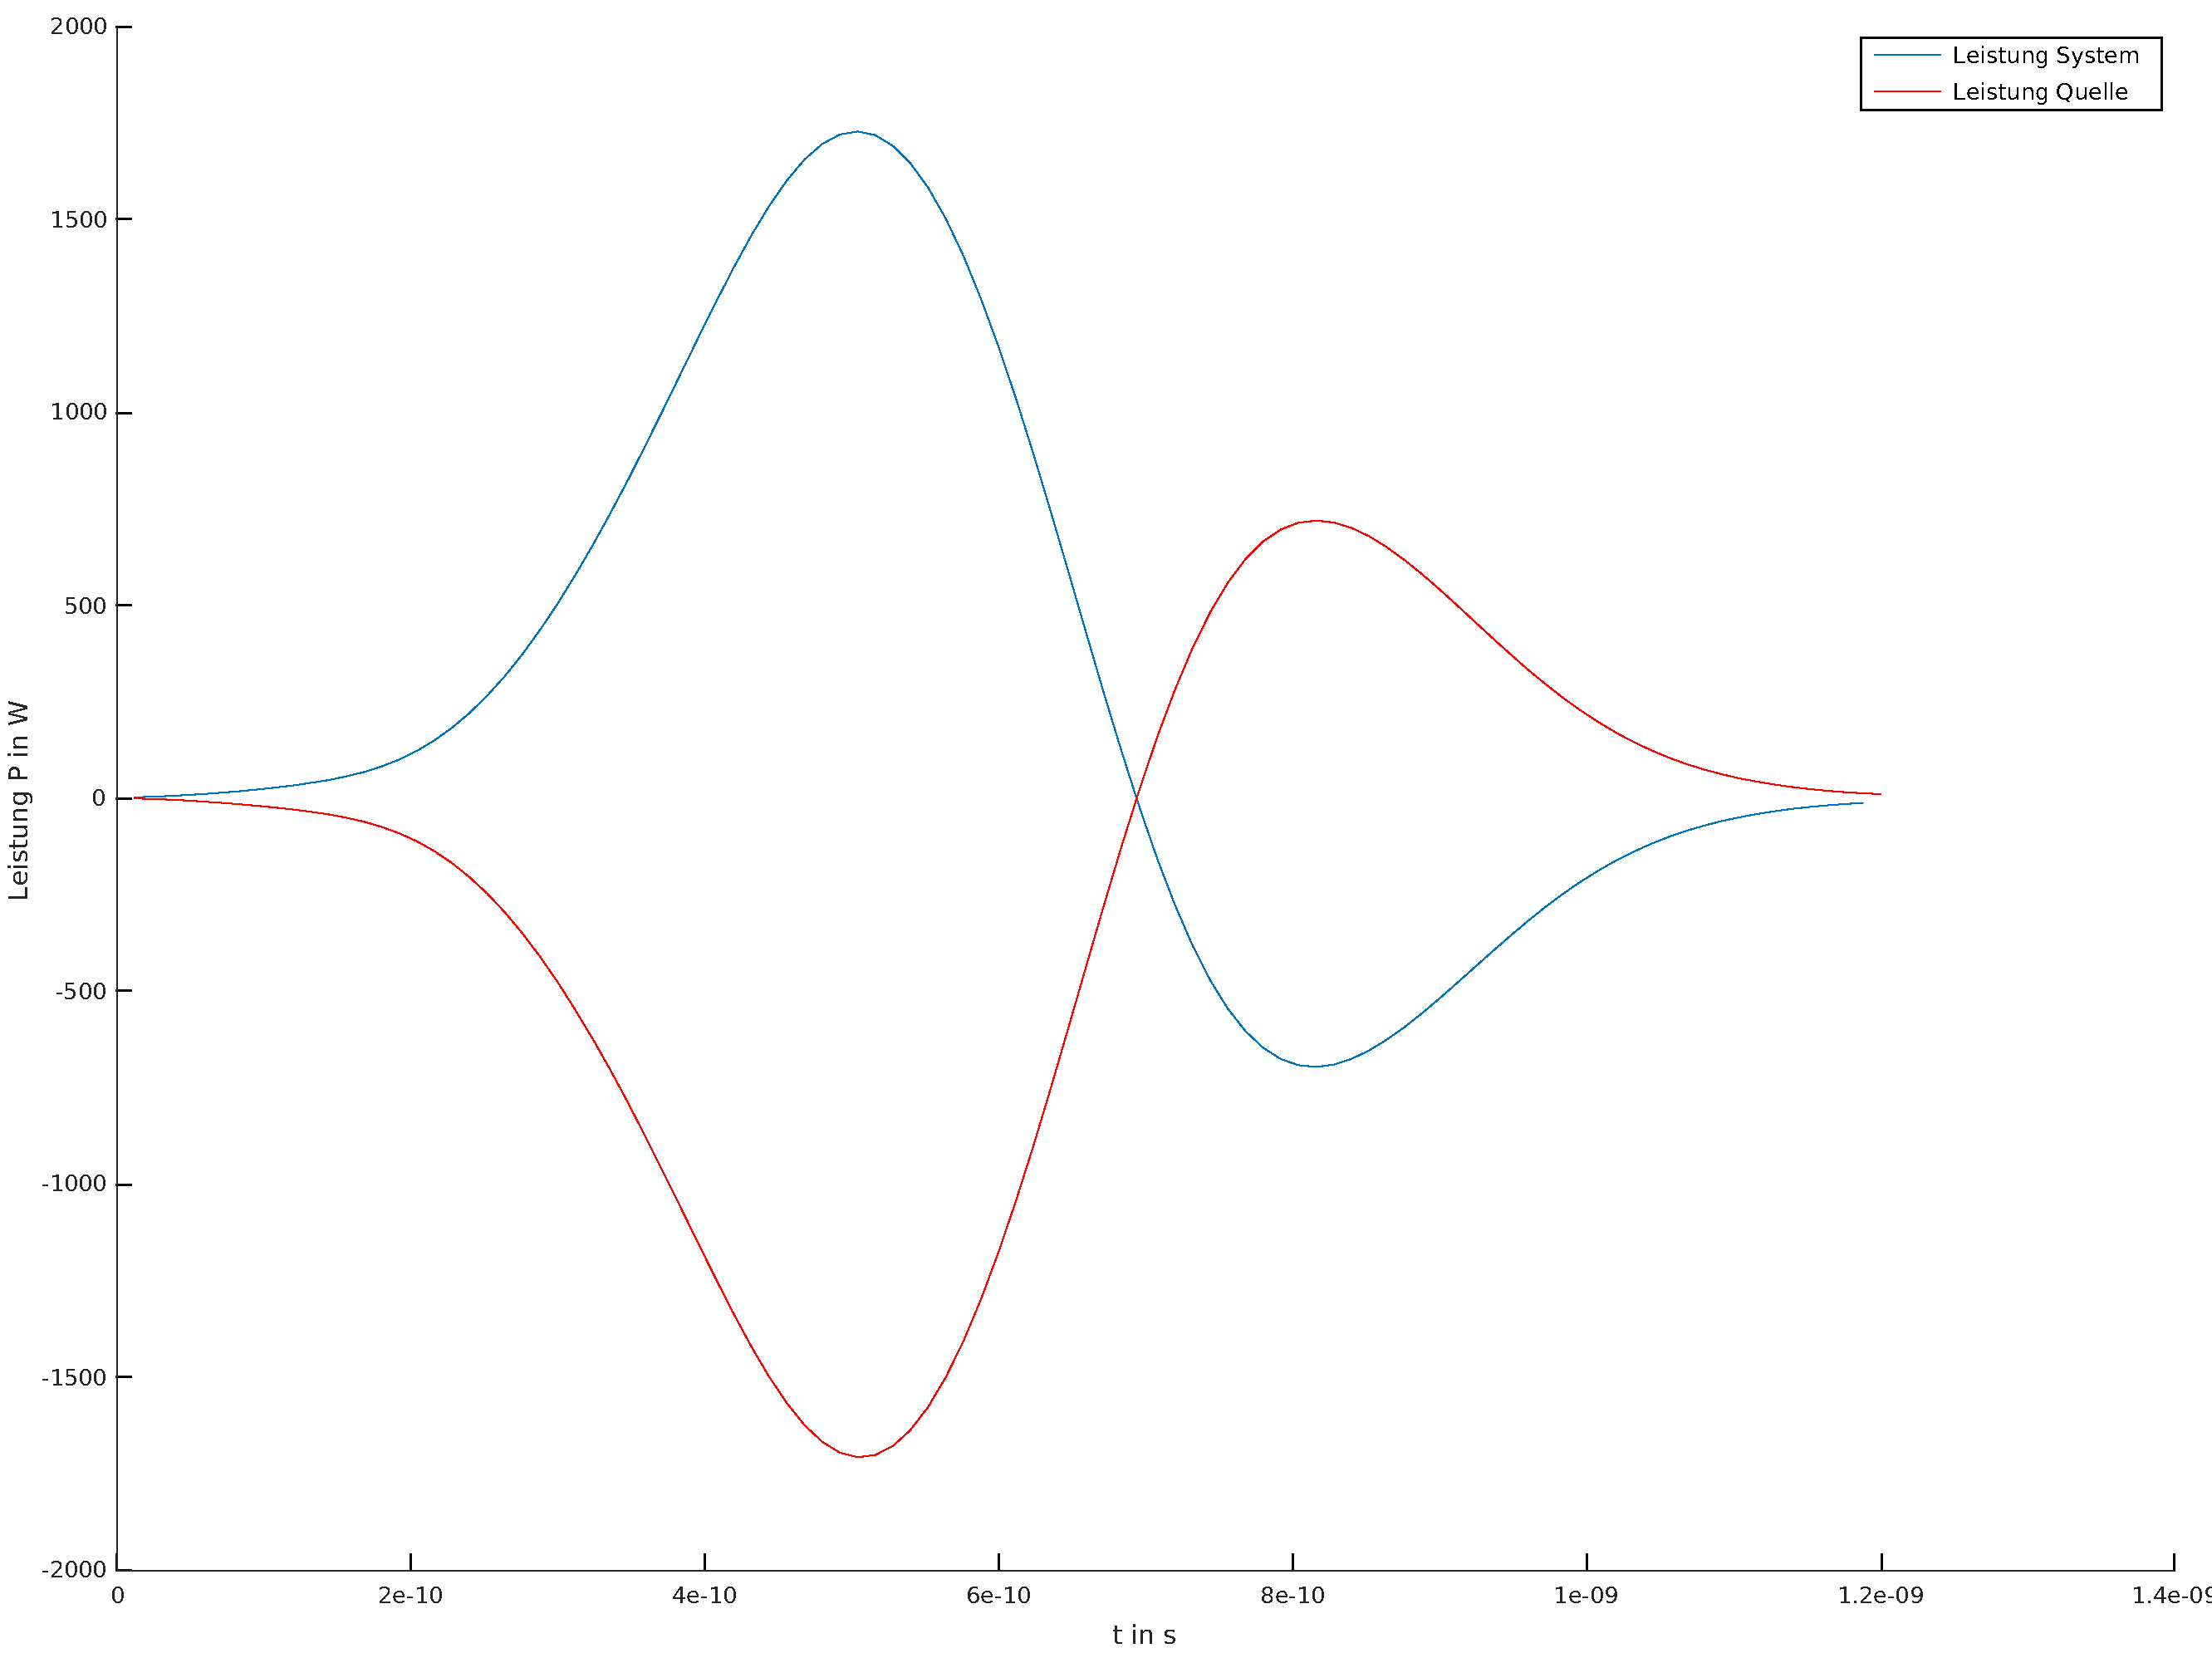
\includegraphics[width=0.7\linewidth]{Leistung}
	\caption{Leistung des Anregestroms und der Zylinderwelle}
	\label{fig:leistung}
\end{figure}


%\emph{Fügen Sie hier Ihre Lösung ein}



\section{Fazit}
\emph{Fügen Sie hier Ihre Lösung ein}

\end{document}
